\documentclass[10pt]{standalone}
\usepackage[utf8]{inputenc}
\usepackage{pgf,tikz}
\usetikzlibrary{arrows}
\usetikzlibrary{arrows.meta}
\pagestyle{empty}
\begin{document}
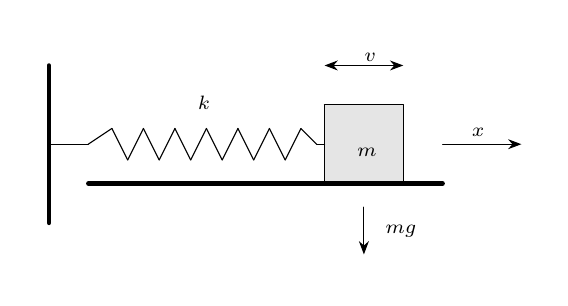
\begin{tikzpicture}[line cap=round,line join=round,>=Stealth,x=1.0cm,y=1.0cm]
\clip(-0.27,-0.7) rectangle (6.24,2.48);
\fill[fill=black,fill opacity=0.1] (3.5,1.5) -- (3.5,0.5) -- (4.5,0.5) -- (4.5,1.5) -- cycle;
\draw [line width=1.6pt] (0,0)-- (0,2);
\draw [line width=1.6pt] (0.5,0.5)-- (5,0.5);
\draw (3.5,1.5)-- (3.5,0.5);
\draw (3.5,0.5)-- (4.5,0.5);
\draw (4.5,0.5)-- (4.5,1.5);
\draw (4.5,1.5)-- (3.5,1.5);
\draw (0,1)-- (0.5,1);
\draw (0.5,1)-- (0.8,1.2);
\draw (0.8,1.2)-- (1,0.8);
\draw (1,0.8)-- (1.2,1.2);
\draw (1.2,1.2)-- (1.4,0.8);
\draw (1.4,0.8)-- (1.6,1.2);
\draw (1.6,1.2)-- (1.8,0.8);
\draw (1.8,0.8)-- (2,1.2);
\draw (2,1.2)-- (2.2,0.8);
\draw (2.2,0.8)-- (2.4,1.2);
\draw (2.4,1.2)-- (2.6,0.8);
\draw (2.6,0.8)-- (2.8,1.2);
\draw (2.8,1.2)-- (3,0.8);
\draw (3,0.8)-- (3.2,1.2);
\draw (3.2,1.2)-- (3.4,1);
\draw (3.4,1)-- (3.5,1);
\draw [->] (5,1) -- (6,1);
\draw [->] (4,0.2) -- (4,-0.4);
\draw [->] (4,2) -- (4.5,2);
\draw [->] (4,2) -- (3.5,2);
\begin{scriptsize}
\draw[color=black] (4.04,0.9) node {$m$};
\draw[color=black] (1.97,1.52) node {$k$};
\draw[color=black] (5.45,1.15) node {$x$};
\draw[color=black] (4.47,-0.11) node {$mg$};
\draw[color=black] (4.08,2.1) node {$v$};
\end{scriptsize}
\end{tikzpicture}
\end{document}